\documentclass{beamer}
%Information
\title{Algebra 2: Sequnence and Inequalities}
\titlegraphic{\hfill
\includegraphics[height=1cm]{orange.png}}
\institute{Youth STEM Academy}
\author{Erzhuo Wang}
\date{July 18,2024}
%Theme
\usetheme[block=fill, sectionpage=none]{metropolis}
\useoutertheme{infolines}
\useinnertheme{metropolis}
\setbeamertemplate{blocks}[rounded][shadow=false]
\setbeamertemplate{items}[ball]
\setbeamertemplate{sections/subsections in toc}[ball]
\setbeamertemplate{headline}{}
\logo{YSA}
\usecolortheme{custom}
%\usetheme{Madrid}
%\usetheme{Heverlee}

%Setting
\usepackage[UTF8,noindent]{ctexcap}
\theoremstyle{definition}
\newtheorem{defn}{Definition}[section]
\newtheorem{coro}[defn]{Corollary}
\newtheorem{theo}[defn]{Theorem}
\newtheorem{exer}[defn]{Exercise}
\newtheorem{rema}[defn]{Remark}
\newtheorem{lem}[defn]{Lemma}
\newtheorem{prop}[defn]{Proposition}
\newtheorem{nota}[defn]{Notation}
\newtheorem{exam}[defn]{Example}
\newtheorem{ques}[defn]{Question}

\newenvironment{prooff}{{\noindent\it\textcolor{cyan!40!black}{Proof}:}\,}{\par}
\newenvironment{proofff}{{\noindent\it\textcolor{cyan!40!black}{Proof of the lemma}:}\,}{\qed \par}
\newcommand{\bbrace}[1]{\left\{ #1 \right\} }
\newcommand{\bb}[1]{\mathbb{#1}}
\newcommand{\p}{^{\prime}}
\renewcommand{\mod}[1]{(\text{mod}\,#1)}
\newcommand{\blue}[1]{\textcolor{blue}{#1}}
\newcommand{\spec}[1]{\text{Spec}({#1})}
\newcommand{\rarr}[1]{\xrightarrow{#1}}
\newcommand{\larr}[1]{\xleftarrow{#1}}
\newcommand{\emptyy}{\underline{\quad}}
\newenvironment{enu}{\begin{enumerate}[(1)]}{\end{enumerate}}
%ctrl+点击文本返回代码  选中代码 ctrl+alt+j 为代码查找文本
\begin{document}
\begin{frame}
    \titlepage
\end{frame}
\begin{frame}{Arithmetic Sequence and Geometric Sequnence}
    \begin{defn}
        The sequence $a_1,\dots,a_n,\dots$ is arithemetic if there is a constant $d$ such that $a_n-a_{n-1}=d$ for
        $n=2,3,4,\dots$.(算术序列/等差数列)

        The sequence $b_1,b_2\dots,b_n$ is geometric if there is a constant $r\neq 0$ such that $\frac{b_n}{b_{n-1}}=r$.(等比数列)
    \end{defn}
    \begin{exam}
        $a_n=3n+5$ is a arithemetic sequence and $b_n=(-1)^n$ is a geometric Sequnence
    \end{exam}
\end{frame}
\begin{frame}{Partial Sum(部分和公式)}
    \begin{theo}[Partial Sum of $a_n$ and $b_n$]
        If $a_1, a_2, a_3, \cdots, a_n, \cdots$ is an arithmetic sequence with the common difference $d$, then
        $a_n=a_1+(n-1) d$, where $a_n$ is the $n$-th term
        $$S_n=\frac{\left(a_1+a_n\right) n}{2}$$,
        where $s_n$ is the partial sum of its first $n$ terms.

        If $a_1, a_2, a_3, \cdots, a_n, \cdots$ is a geometric sequence with the common ratio $r$, then
        $a_n=a_1 r^{n-1}$, where $a_n$ is the $n$-th term
        $$s_n=\frac{a_1\left(1-r^n\right)}{1-r}$$,
        where $s_n$ is the partial sum of its first $n$ terms.

    \end{theo}
\end{frame}
\begin{frame}{Exercise}
    \begin{ques}
        The sum of the odd positive integers from $1$ to $n$ is 9409, What is $n$?

        从$1$到$n$的奇数正整数的和是9409,$n$是多少?
    \end{ques}
    \begin{ques}[AMC 8,2016-19]
        The sum of $25$ consecutive even integers is $10000$. What is the largest of these
        $25$ consecutive integers?

        $25$个连续偶数的和是$10000$, 求其中最大的那个.
    \end{ques}
    \begin{ques}
        Four numbers are written in a row. The average of the first two is 21 , the average of the middle two is 26 , and the average of the last two is 30 . What is the average of the first and last of the numbers?
        
        (A) 24 (B) 25 (C) 26 (D) 27 (E) 28
    \end{ques}
\end{frame}
\begin{frame}{Exercise}
    \begin{ques}[AMC 8, 2023-25]
        Fifteen integers $a_1, a_2, a_3, \ldots, a_{15}$ are arranged in order on a number line. The integers are equally spaced and have the property that
        $$
            1 \leq a_1 \leq 10,13 \leq a_2 \leq 20, \text { and } 241 \leq a_{15} \leq 250
        $$

        Find the value of $a_{14}$?

        $a_1,a_2,\dots,a_{15}$ 为一个等差数列, 且这15个数都是整数, 满足如下不等式:
        $$
            1 \leq a_1 \leq 10,13 \leq a_2 \leq 20, \text { and } 241 \leq a_{15} \leq 250
        $$
        求$a_{14}$.
    \end{ques}
\end{frame}
\begin{frame}{Perfect Cubes}
\begin{ques}[AMC 8, 2018-25]
    考虑数列$a_n=n^3$, 请问有多少个$n$使得$2^8+1\le a_n\le 2^{18}+1$.
\end{ques}
\end{frame}
\begin{frame}{Some Useful Results(一些求和技巧)}
    \begin{align*}
        \sum_{i=1}^n i^2 & =1^2+2^2+3^2+\cdots+n^2=\frac{n(n+1)(2 n+1)}{6}         \\
        \sum_{i=1}^n i^3 & =1^3+2^3+3^3+\cdots+n^3=\left(\frac{n(n+1)}{2}\right)^2
    \end{align*}
    \begin{equation*}
        \sum_{i=1}^n \frac{1}{i(i+1)}=1-\frac{1}{n+1}
    \end{equation*}
\end{frame}
\begin{frame}{不等式的基本性质}
    \begin{itemize}
        \item $a^2\ge 0$
        \item 若$a>b$, 且$c>d$,则$a+c>b+d$.
        \item 若$a>b$, 且$c>0$, 则$ac>bc$, 若$a>b$, 且$c<0$, 则$ac<bc$.
    \end{itemize}
\end{frame}
\begin{frame}{A/G Mean Inequality(算术/几何 均值不等式)}
    \begin{theo}
       For $a,b\ge 0$, 
       \begin{equation*}
          \sqrt{ab}\le \frac{a+b}{2}
       \end{equation*}
    \end{theo}
    \begin{exam}
        Find the greatest possible value of the product $xy$, where $x,y$ are positive real numbers with $x+2y=12$.
    \end{exam}
\end{frame}
\begin{frame}{Baskets}
    Steph scored 15 baskets out of 20 attempts in the first half of a game, and 10 baskets out of 10 attempts in the second half. Candace took 12 attempts in the first half and 18 attempts in the second. In each half, Steph scored a higher percentage of baskets than Candace. Surprisingly they ended with the same overall percentage of baskets scored. How many more baskets did Candace score in the second half than in the first?
    
    \begin{tabular}{l|c|c} 
    & First Half & Second Half \\
    \hline Steph & $\frac{15}{20}$ & $\frac{10}{10}$ \\
    Candace & $\frac{\Box}{12}$ & $\frac{\Box}{18}$
    \end{tabular}
    
    (A) 7 (B) 8 (C) 9 (D) 10 (E) 11
\end{frame}
\begin{frame}{Solution}
    Let $x$ be the number of shots that Candace made in the first half, and let $y$ be the number of shots Candace made in the second half. Since Candace and Steph took the same number of attempts, with an equal percentage of baskets scored, we have $x+y=10+15=25$. In addition, we have the following inequalities:

$$
\frac{x}{12}<\frac{15}{20} \Longrightarrow x<9
$$

and

$$
\frac{y}{18}<\frac{10}{10} \Longrightarrow y<18
$$


Pairing this up with $x+y=25$ we see the only possible solution is $(x, y)=(8,17)$, for an answer of $17-8=(\mathbf{C}) 9$.
\end{frame}
% \begin{frame}{Exercise}
% \begin{ques}
%     求函数 $x+\frac{1}{x},x>0$ 和 $x(4-2x), 0<x<2$的最大值.
% \end{ques}
% \begin{ques}
%     Find the maximum possible value of $\frac{x}{1+x+x^2}$ as $x$ ranges over the positive real numbers.

%     求函数
%     \begin{equation*}
%         \frac{x}{1+x+x^2}, x\in \bb{R}_{>0}
%     \end{equation*}
%     最大值
% \end{ques}
% \end{frame}
% \begin{frame}{Cauchy Inequality}
% \begin{theo}
%     For natural number $n$, let $a_1, a_2, a_3, \cdots, a_n$ and $b_1, b_2, b_3, \cdots, b_n$ be two sequences of $n$ real numbers. Then
%     $$
%     (\sum_{i=1}^n a_ib_i)^2 \le (\sum_{i=1}^n a_i^2)(\sum_{i=1}^n b_i^2)
%     $$
    
%     Moreover, equality occurs only when the one of the two sequences $a_1, a_2, a_3, \cdots, a_n$ and $b_1, b_2, b_3, \cdots, b_n$ is a multiple of the other, that is, there are numbers $x$ and $y$ so that $x a_j=y b_j$ for every $j=1,2,3, \ldots n$.
% \end{theo}
% \end{frame}
% \begin{frame}{Homework}
%     \begin{ques}[AMC 8, 2023-25]
%         Fifteen integers $a_1, a_2, a_3, \ldots, a_{15}$ are arranged in order on a number line. The integers are equally spaced and have the property that
%         $$
%             1 \leq a_1 \leq 10,13 \leq a_2 \leq 20, \text { and } 241 \leq a_{15} \leq 250
%         $$

%         Find the value of $a_{14}$?

%         $a_1,a_2,\dots,a_{15}$ 为一个等差数列, 且这15个数都是整数, 满足如下不等式:
%         $$
%             1 \leq a_1 \leq 10,13 \leq a_2 \leq 20, \text { and } 241 \leq a_{15} \leq 250
%         $$
%         求$a_{14}$.
%     \end{ques}
% \end{frame}
\begin{frame}{Homework}
    \begin{ques}[AMC 8, 2023-22]
        In a sequence of positive integers, each term after the second is the product of the previous two terms. The sixth term is 4000 . What is the first term?
        (A) 1 (B) 2 (C) 4 (D) 5 (E) 10
    \end{ques}
    \begin{ques}[AMC 8, 2023-20]
        Two integers are inserted into the list $3,3,8,11,28$ to double its range. The mode(众数) and median(中位数) remain unchanged. What is the maximum possible sum of the two additional numbers?
          
        (A) 56 (B) 57 (C) 58 (D) 60 (E) 61
    \end{ques}
\end{frame}
\begin{frame}
    \begin{figure}
        \centering
        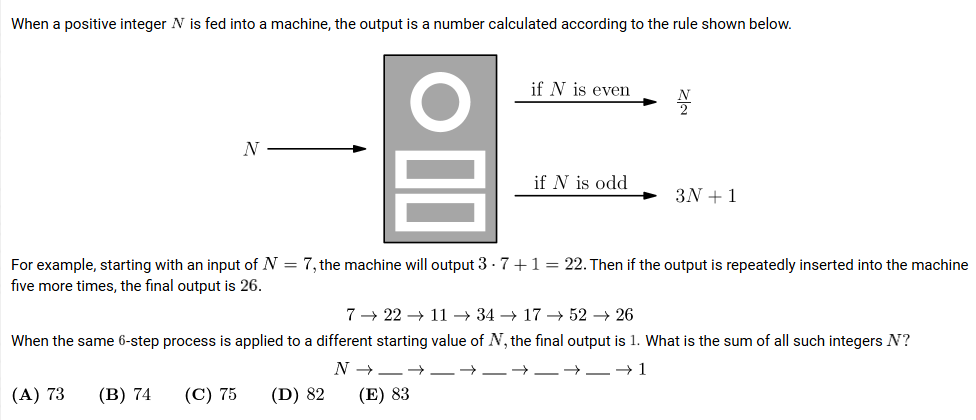
\includegraphics[width=1\textwidth]{3n+1.png}
    \end{figure}
\end{frame}
\end{document}